% article example for classicthesis.sty
\documentclass[12pt,letter]{article} % KOMA-Script article scrartcl
\usepackage{lipsum}     %lorem ipsum text
\usepackage{titlesec}   %Section settings
\usepackage{titling}    %Title settings
\usepackage[margin=10em]{geometry}  %Adjusting margins
\usepackage{setspace}
\usepackage{listings}
\usepackage{amsmath}    %Display equations options
\usepackage{amssymb}    %More symbols
\usepackage{xcolor}     %Color settings
\usepackage{pagecolor}
\usepackage{mdframed}
\usepackage[utf8]{inputenc}
\usepackage{longtable}
\usepackage{multicol}
\usepackage{graphicx}
\usepackage{url}
\graphicspath{ {./Images/} }
\setlength{\columnsep}{1cm}

% ====| color de la pagina y del fondo |==== %
\pagecolor{white}
\color{black}



\begin{document}
    %========================{TITLE}====================%
    \title{\rmfamily\normalfont{ 4th Lab  }}
    \author{{Juan Esteban Murcia y Rodrigo Castillo}}
    \date{\today}

    \maketitle


    %=======================NOTES GOES HERE===================%

    \section{Static Analysis}
        \subsection{Get the hash of the malware and search for it in Virus
            Total. Is is recognized as a malware for some antivirus?}
                The library outlook.dll is recognized by virustotal as a malware by
                $ 59/70  $ antiviruses.
                \begin{figure}[h]
                    \centering
                    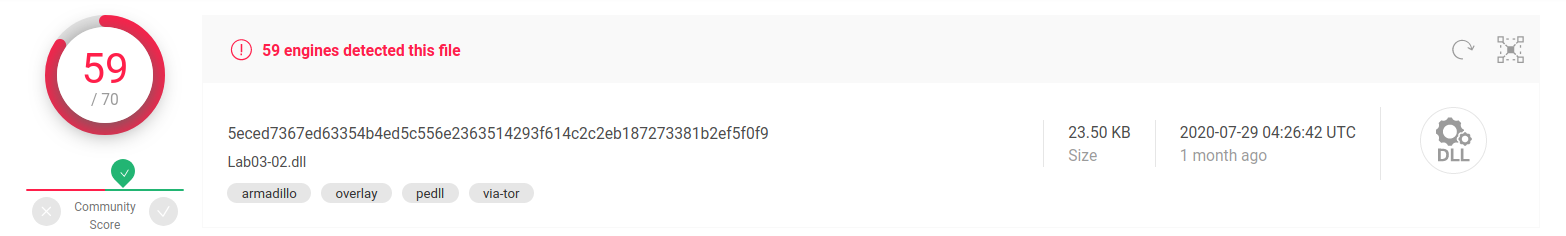
\includegraphics[width=0.8\linewidth]{hash.png}
                    \caption{Hash}
                    \label{hash}
                \end{figure}

        \subsection{Analyze the strings using the command line tool "Strings".
        Which are the strings more suspicious and why?}

            \begin{figure}[h!]
                \centering
                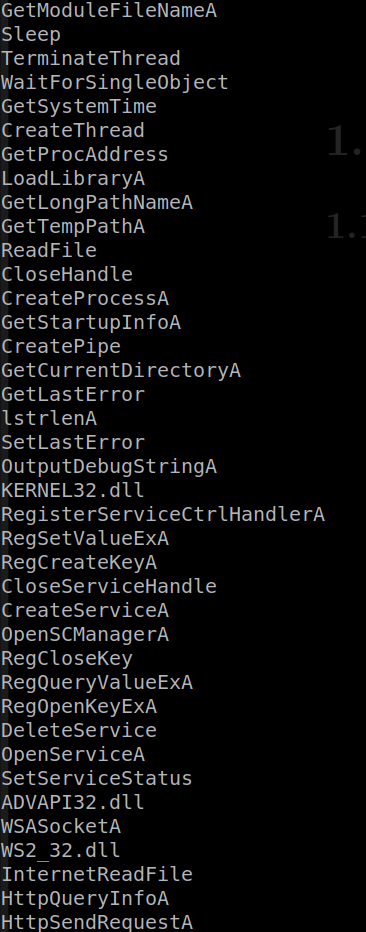
\includegraphics[width=0.4\linewidth]{strings.png}
                \caption{Strings}
                \label{strings}
            \end{figure}
            inside the list we can find the library $ kernel32.dll  $ which is
            really powefull, also, we can see that is importing $ sleep  $
            library, that means that the malware probably is not going to
            execute inmediatly , sometimes, malwares are programmed with delay
            with the prupose of being sneaky. Also, it's importing functions
            for installing processes like $ installA  $ , $ install  $ ... etc,
            its also importing libraries for networking
            , this can be used by the malware for remotely installing processes later.
            there is a library that is interesting not because of its
            potential but it talks about the way that the program was made, the
            library $ malloc  $ it's a $ C  $ library, that means that the
            pogram was made in C or C++.
            \\ the malware is also connecting to an attacker's localhost in $
            practicalmalwareanalysis.com  $ .

        \subsection{Is the malware packed? Analyze it with PEiD. Unpack if possible.}
            the malware is not packed but its a c++ program .\\
            \begin{figure}[h!]
                \centering
                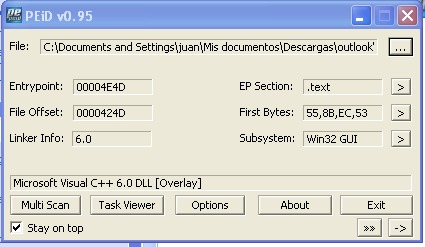
\includegraphics[scale=0.5]{Peid.jpeg}
                \caption{PEid}
                \label{fig:Peid}
            \end{figure}$ $\\

        \subsection{Analyze the PE with PEView and review detailed the "text",
        "data", "rdata" and "resource" sections (Use "Resource Hacker" to
        access to the resource section). What information is useful from theses
        sections?}\pagebreak
		\begin{figure}[h!]
			\centering
			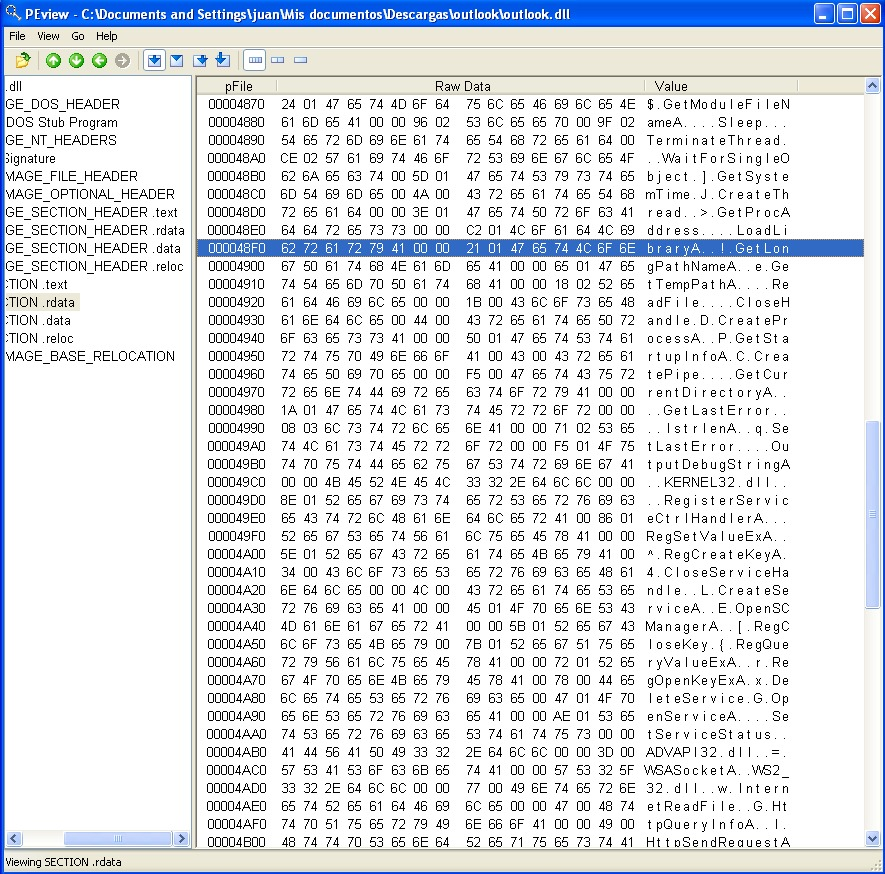
\includegraphics[scale=0.28]{img1.jpeg}
			\caption{Rdata}
			\label{libraries}
		\end{figure}
		\begin{figure}[h!]
			\centering
			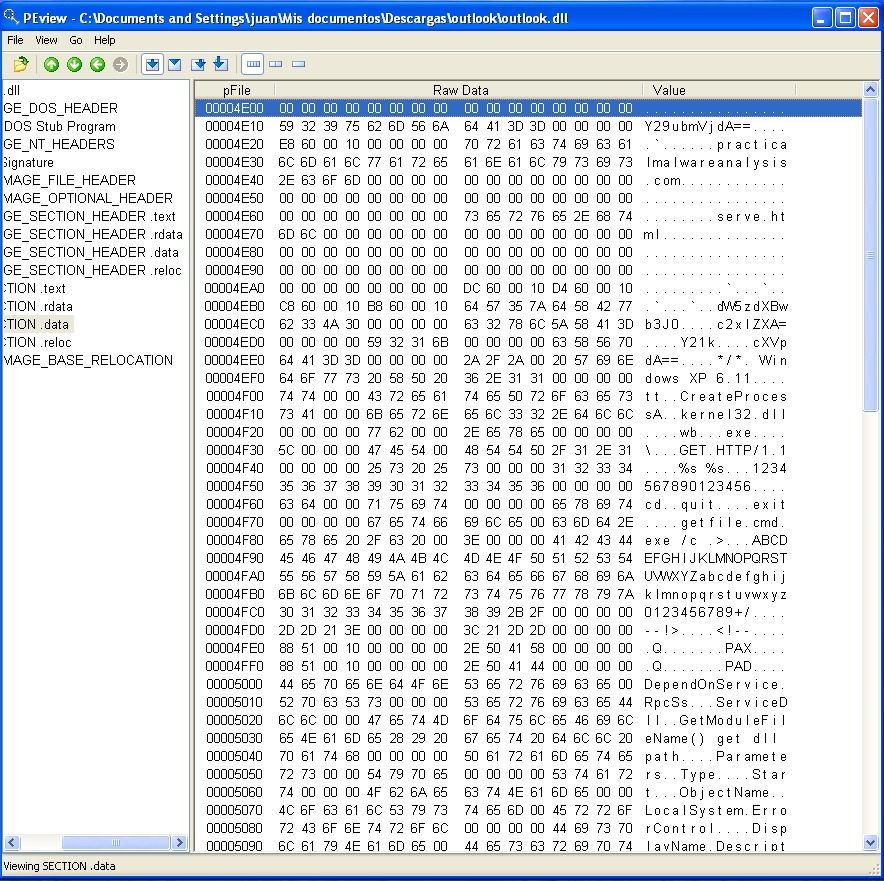
\includegraphics[scale=0.28]{img2.jpeg}
		\end{figure}
		\begin{figure}[h!]
			\centering
			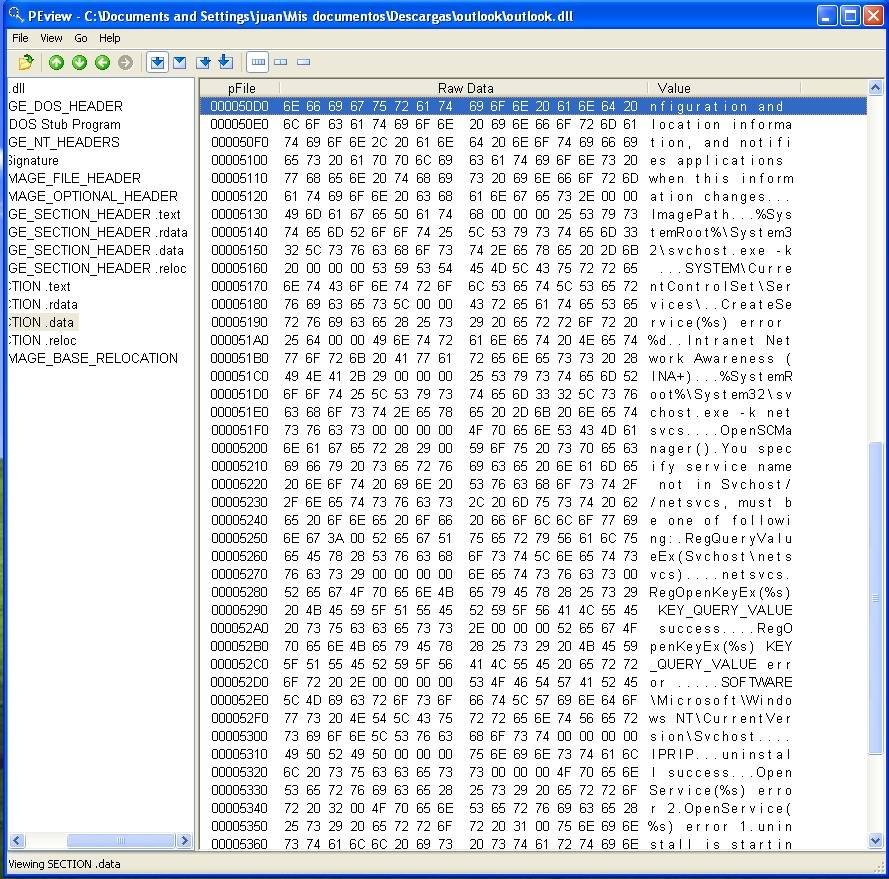
\includegraphics[scale=0.28]{img3.jpeg}
			\caption{data and text sections}
			\label{5}
		\end{figure}$ $
		\pagebreak$ $\\
		Clearly in this images we can find really important information, like how the malware is opening and using registry keys, create a host service with the name of IPRIP, adding all the dynamic libraries and functions the malware seems to be using.
        \subsection{When the file was compiled?}
            the file was created on $ 2010:09:27 20:00:25-05:00  $
            \begin{figure}[h!]
            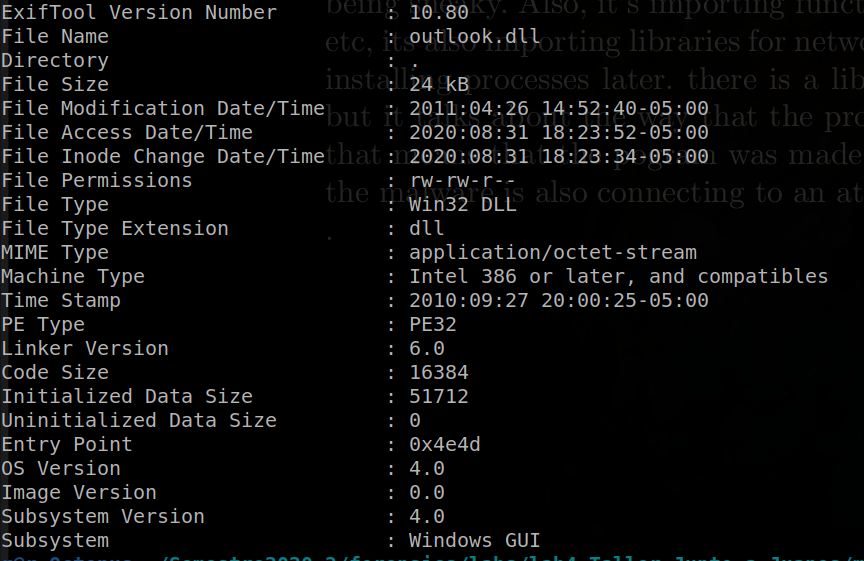
\includegraphics[width=0.8\linewidth]{exif.png}
            \end{figure}

        \subsection{Which imported libraries and functions can be seen from the static analysis?}
            those are the libraries and functions that the program is importing.
            \\
            from here, we can see very important information such as the keys
            that the malware is creating, here there are the imported
            libraries:
            \begin{figure}[h!]
            	\centering
            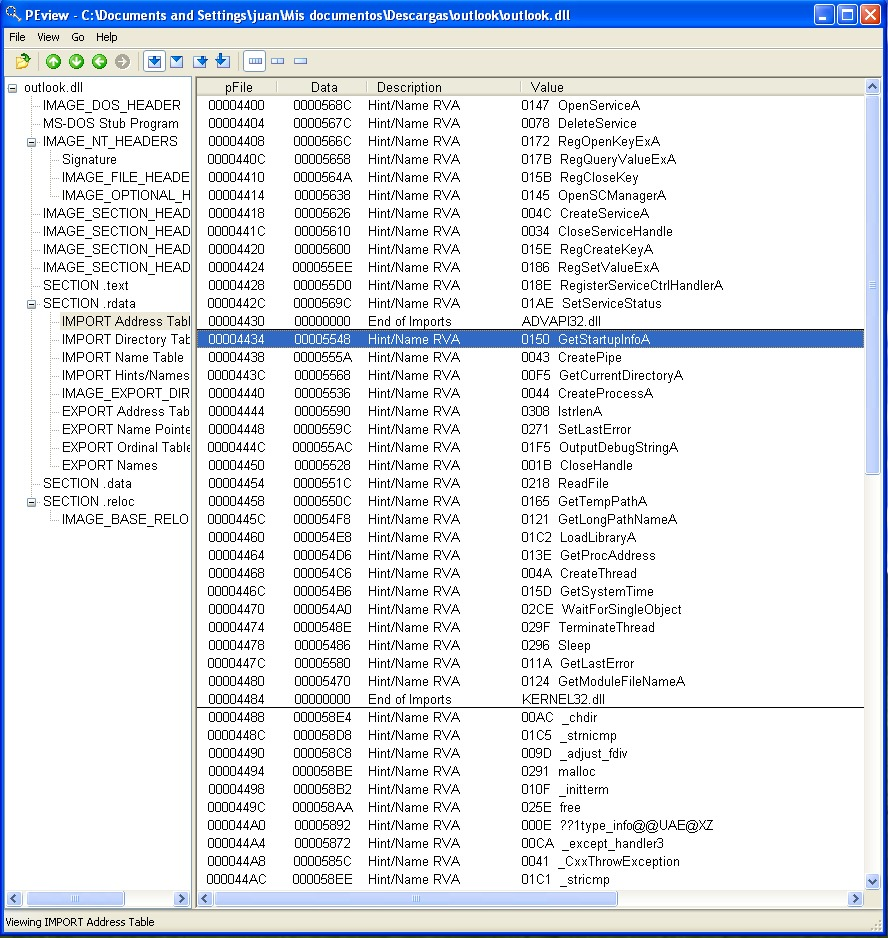
\includegraphics[width=0.5\linewidth]{imports2.jpeg}
            \end{figure}
		$ $\\
		\pagebreak
        \subsection{There is some exports?}
            yes, there are exports. it exports several functions  that seems to
            have installing and uninstalling purposes.

            \begin{figure}[h!]
        	    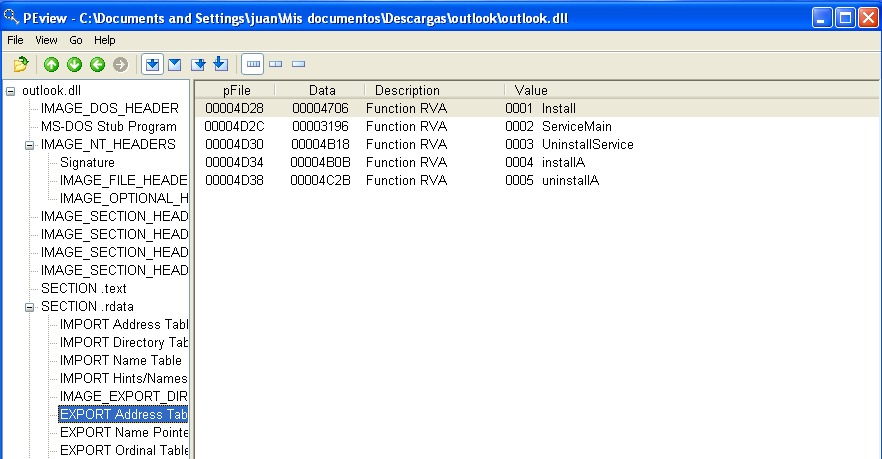
\includegraphics[width=0.8\linewidth]{exports1.jpeg}
            \end{figure}
			 \pagebreak

        \subsection{What may be the functionalities of the malware?}
            My partner and I think that the malware its a dropper, because it
            has the capability of install processes that it's going to use
            later. it also has the capability of create network services using
            the $ srvhost  $  process. this can mean that an attacker ($
            practicalmalwareanalysis  $ ) can install other programs in the
            victim's machine.

        \subsection{From all previous answers, identify all host-based signatures for this malware.}
        The next information is all the host based signatures virustotal.com identified, but that we also identified with the static analysis, all these signatures are based on how the malware behaves inside an infected machine, which libraries it import, which functions it exports, among other characteristics.
            processes:
            \\ 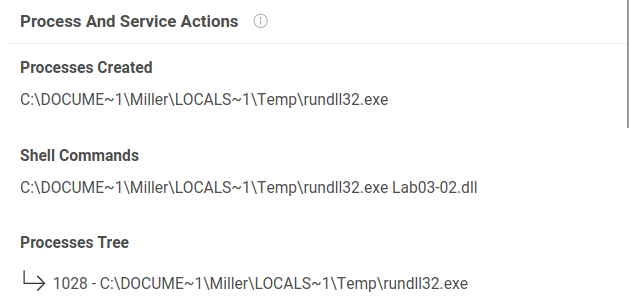
\includegraphics[width=0.5\linewidth]{procesos.png}
            \\modules :
            \\ 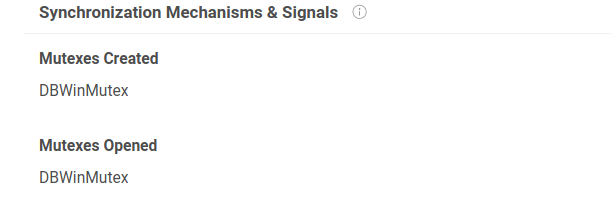
\includegraphics[width=0.5\linewidth]{modules.png}
            \\ runtime modules :
            \\ 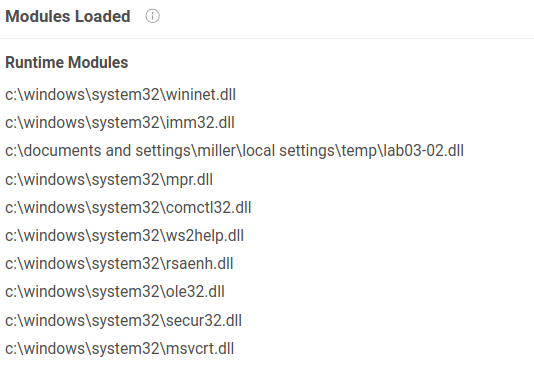
\includegraphics[width=0.8\linewidth]{runtime.png}
            \\

        \subsection{From all previous answers, identify all antivirus signatures for this malware.}
        	As virustotal.com and we identified, the following information related to the presentation of the malware, however these characteristics can be easily modified by an attacker. Information like its hash values, its size, the names it might have, etc.
            hashes :\\
            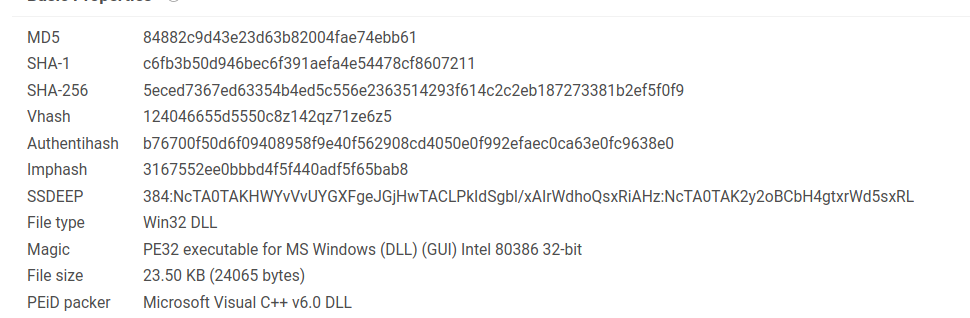
\includegraphics[width=0.8\linewidth]{hashes.png}
            \\ names
            \\ 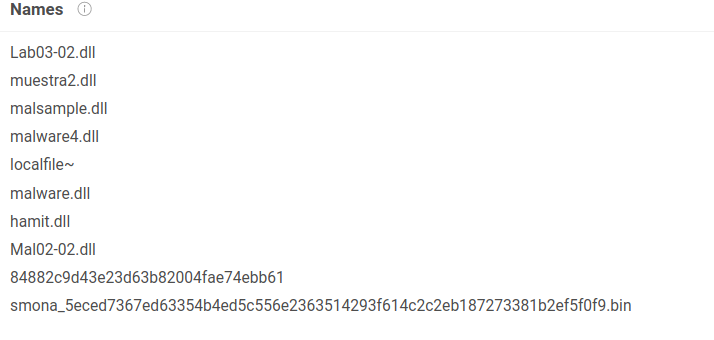
\includegraphics[width=0.8\linewidth]{names.png}
            \\ history
            \\ 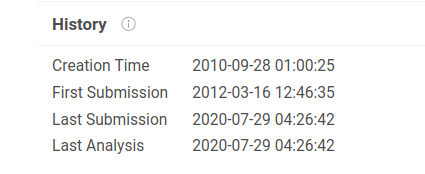
\includegraphics[width=0.8\linewidth]{hist.png}

        \subsection{From all previous answers, identify all network-based signatures for this malware.}
        Finally, as we can check in the first image if the figure \ref{5}, the malware has a domain within its data setion, \url{practicalmalwareanalysis.com}, meaning that the malware is probably going to connect to that url, perform a DNS resolution and communicate with a command\&control server.


                            % ====| PENDIENTE A HACERSE CON JUANES!!! |==== %

    \section{Dynamic Analysis}

        \subsection{Take a snapshot of the register keys before the infection using the application Regshot.}
            here is the snapchot of the register keys
            \\
            \begin{figure}[h!]
                \centering
                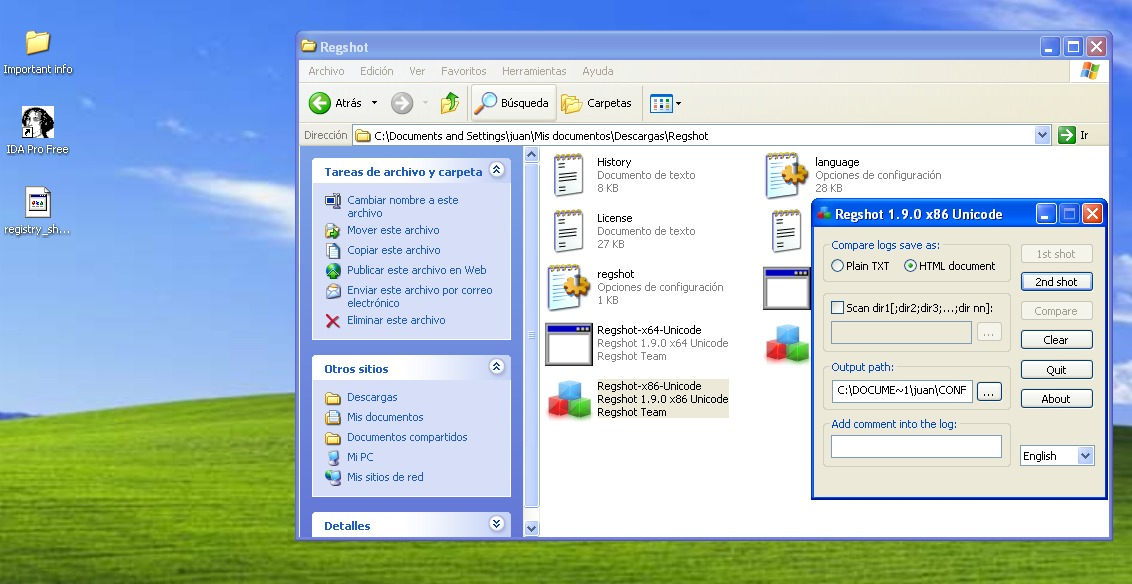
\includegraphics[width=0.5\linewidth]{punto1.jpeg}
                \caption{snapchot of the register keys}
                \label{snapchot register keys}
            \end{figure}
            \\

        \subsection{Take a snapshot of the virtual machine before the infection}
            here is the snapchot of the virtual machine before the infection  :
            \\
            \begin{figure}[h!]
                \centering
                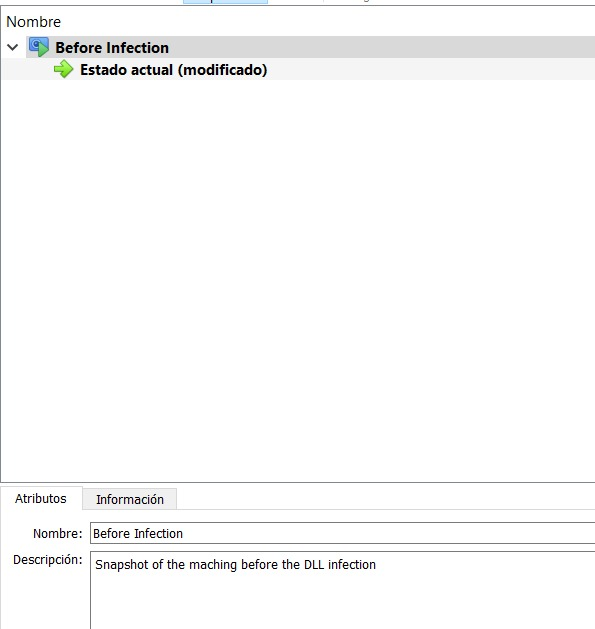
\includegraphics[width=0.5\linewidth]{punto2.jpeg}
                \caption{snapchot}
                \label{snapchot of the virtual machine before the infection}
            \end{figure}
            \\

        \subsection{Install the malware using the command: C:\>rundll32.exe outlook.dll, installA}
            installing the malware using the command  $ C:\>rundll32.exe outlook.dll  $
            \\
            \begin{figure}[h!]
                \centering
                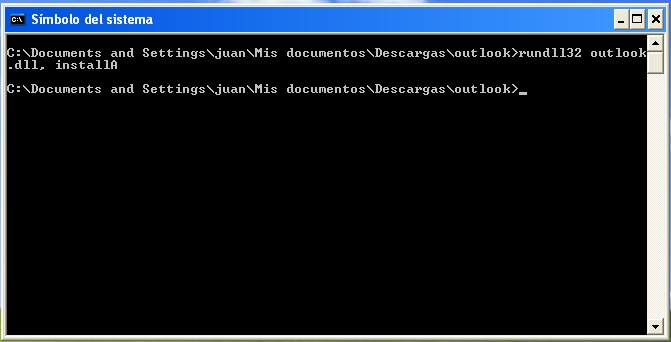
\includegraphics[width=0.5\linewidth]{punto3.jpeg}
                \caption{command}
                \label{command execution:}
            \end{figure}
            \\

        \subsection{installA was a function identified previously in the static
        analysis?}
            Yes, installA was a function we identified with the static analysis
            in the strings and in the exports.

        \newpage
        \subsection{Take a second snapshot of the register keys with Regshot.
        Identify the changes before and after the infection (keys created,
        modified, delete, etc)?}

            \\
            \begin{figure}[h!]
                \centering
                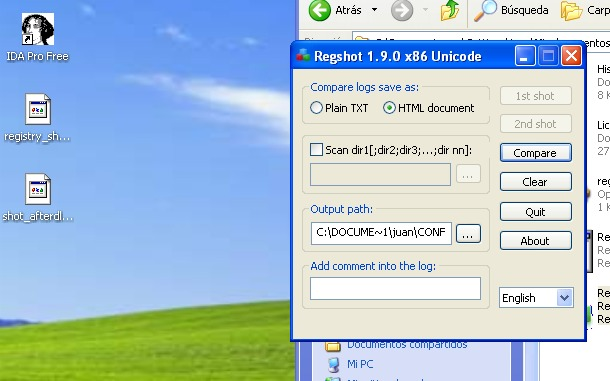
\includegraphics[width=0.4\linewidth]{punto5_1.jpeg}
                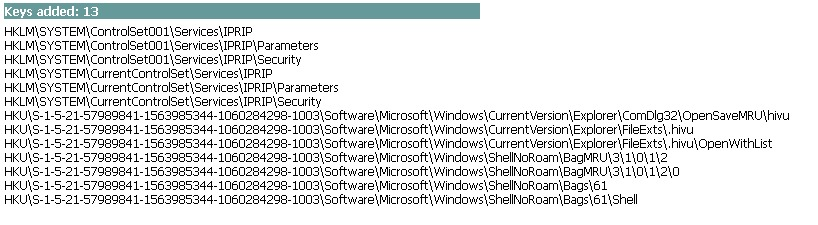
\includegraphics[width=0.4\linewidth]{punto5_2.jpeg}
                \\
                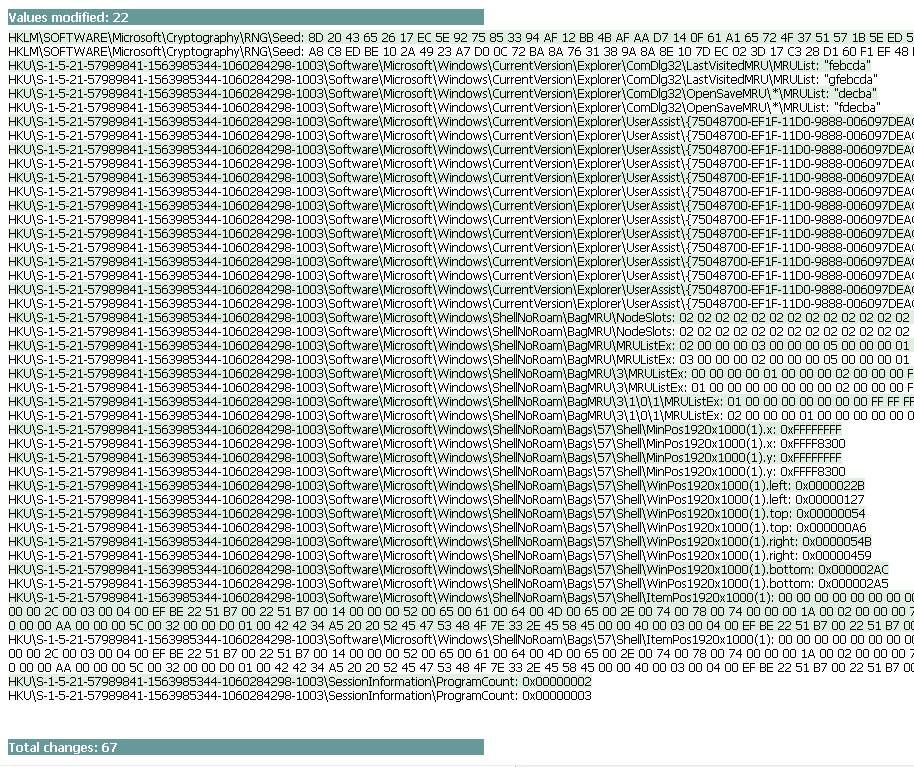
\includegraphics[width=0.4\linewidth]{punto5_3.jpeg}
                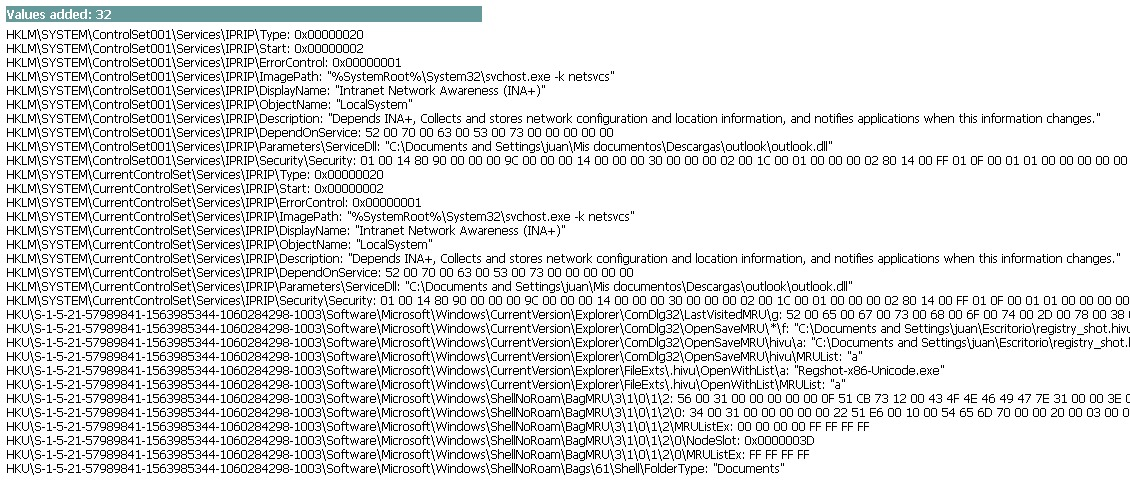
\includegraphics[width=0.4\linewidth]{punto5_4.jpeg}
                \caption{snapchots}
                \label{snapchots snapchots... }
            \end{figure}

            \begin{itemize}
                \item {We can see that it included 13 new keys, and a good amount of them
            involve the new service IPRIP .}
            \item {A total of 22 keys values were modified, however the purpose of the
            modification can't be understood.}
            \item {And finally the infected dll added a total of 32 values to
            exsisting or new keys, most of these new values are for the IPRIP
            service.}
            \end{itemize}

        \subsection{Analyze in detail the register keys and identify the name
        of the service that was installed by the malware?}

            As we identified in the last point, the service the
            malware created is IPRIP, we know it is a service because it was
            located in the service path and it seems to uses the svchost.exe
            executable, that hosts the services of the machine

        \subsection{Analyze the register keys and identify the name of the
        executable that apparently consume (import) the DLL?}
            it is importing service host ,  It includes processes including
            Windows Auto Update and many required system services would be
            running in it. this cat let the attacker control processes and
            windows versions in the victims machine.

        \subsection{ Create a virtual network of 2 Virtual machines. One of
        them will be the infected machine, and the other will be the server of
        Command & Control. Install Netcat on the last one to emulate the behavior
        of a web server.}
        on the command and control machine ...
        \\ 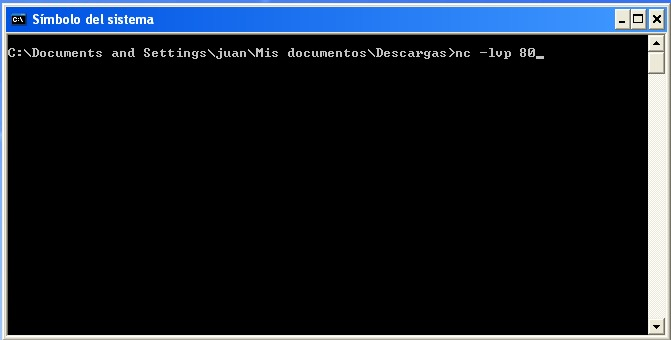
\includegraphics[width=0.5\linewidth]{ncliste.jpeg}
        \\
        on the victim's machine ...
        \\ 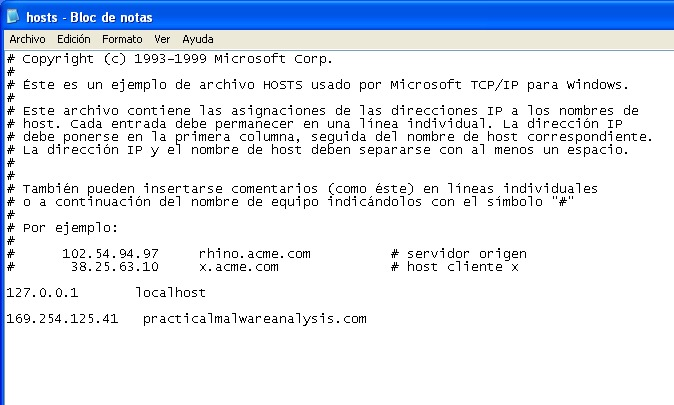
\includegraphics[width=0.5\linewidth]{ncvictim.jpeg}
        \\

        \subsection{Start the malicious service in the infected machine using
        the command: net start IPRIP}

        \subsection{Why IPRIP? Did you find the word (IPRIP) in some of the
        previous steps?}

        \subsection{Execute Process Explorer. Find the process that is running
        the malware using the "Find DLL" functionality of Process Explorer.
        Identify the Process Id (PID)}

        \subsection{Execute Process Monitor and search the process using the PID}

        \subsection{Create filters to reduce the events to fewer than 10 events
        in the Process Monitor. Use filters that allow to identify keys and
        files modified or created.}

        \subsection{Does the malware resolve some domain? }

        \subsection{Configure the nc tool with port 443, 8000 and 80. Which
        port is contacted on that domain? Capture the request done by the
        malware}

        \subsection{From all previous answers, identify all host-based
        signatures for this malware.}

        \subsection{From all previous answers, identify all antivirus
        signatures for this malware. }

        \subsection{From all previous answers, identify all network-based
        signatures for this malware.}


\end{document}
